\documentclass[11pt]{article}
\usepackage{palatino}
\usepackage{graphicx}
%\usepackage{wrapfig}
\usepackage[top=1in, bottom=1in, left=0.5in, right=0.5in]{geometry}
\newcommand{\BibTeX}{{\sc Bib}\TeX}
\begin{document}
\title{Physics Behind the Simulation: A CS296 Group 19 Report}
\author{Tarun Kathuria \\ 110110028 \\ \texttt{tarunkathuria@gmail.com} \and Rohith Kishan \\ 110050071 \\ \texttt{krsrk@cse.iitb.ac.in} \and Vikash Challa \\ 110050077 \\ \texttt{vikash@cse.iitb.ac.in}}
\date{\today}
\maketitle

\section{Introduction}
\begin{figure}[h!]
\caption{CS296 Dominoes Simulation}
\centering
\includegraphics[width=20cm,height=12cm]{intro}
\end{figure}
When such a Box2D Simulation is observed,it is a spectacular view.
However, behind those impeccable timings and those perfectly orchestrated sequence of events, there is vast and complicated mechanics of solid bodies involved!
This report is basically to provide an insight into the laws of physics governing the ``Rube Goldberg" Box2D simulation as part of our \underline{CS 296 lab 3 assignment}.
We present 3 of the top level blocks defined in the constructor in \emph{dominoes.cpp}. These 3 top level blocks are 3 vital components of the ``Rube Goldberg" simulation. They are: \\
\begin{enumerate}
\item The pendulum that knocks the dominoes off
\item The falling dominoes
\item The revolving platform

\end{enumerate}


\section{Physics behind the simulation}
\subsection{The pendulum that knocks the dominoes off}
\begin{figure}[h!]
\caption{The pendulum knocking down the first domino}
\centering
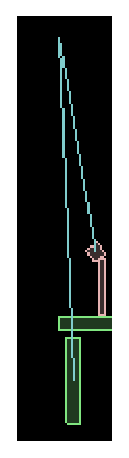
\includegraphics[width=5cm,height=8cm]{pendulum}
\end{figure}
When the simulation starts the pendulum initially makes some angle $\phi$, in $radians$,
 with the vertical, and it then starts moving to the right due to the gravitational force acting on it. Further, suppose that when the pendulum bob is at it's lowest point, it has a velocity of $u$ m/s. When it hits the first domino, it makes an angle $\theta$ with the vertical, say and with velocity $v$ m/s. 
Using the \emph{law of conservation of energy}, we get
\begin{equation}
\frac{1}{2} m v^2 = \frac{1}{2} m u^2 - mgl\cos\theta
\end{equation}
where $m$ is mass of pendulum bob in $kilograms$, $u$ and $v$ are velocities as mentioned above in $metres/{sec}$, $g$ is acceleration due to gravity in $metres/{sec}^2$, $l$ is length of pendulum string in $metres$ and $\theta$ is the angles as mentioned above in $radians$.
\\
Since the mass of a domino is a lot lesser than that of the pendulum bob, using  the \emph{momentum conservation principle}, we get that the initial velocity of the first domino $\approx$  $v$ $metres/sec$.

\subsection{The falling dominoes}
When the pendulum bob hits the first domino, it sets off a beautiful example of rigid body dynamics of the dominoes.
The dominoes are all identical and of height $h$ $metres$, thickness $T$ $metres$ and mass $m$ $kilograms$. 

\begin{figure}[h!]
\caption{Falling dominoes}
\centering
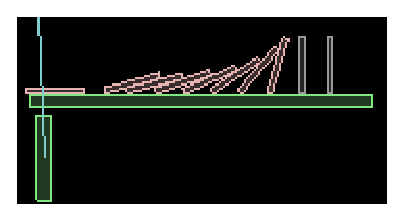
\includegraphics[width=7cm]{dominoes}
\end{figure}

\begin{itemize}
	\item As shown in \textbf{2.1}, the first domino acquires a velocity approximately equal to that of the pendulum bob at the time of impact.
	\item van Leeuwen \cite{DominoEff} makes an approximation that the first domino topples and makes a ``free rotation" till it strikes the second.
	\item After the collision the two fall together till they strike the
	      third and so forth. So we get a succession of rotations and collisions, the two processes
	      being governed by different dynamical laws.
\end{itemize}

\begin{figure}[h!]
\caption{Dominoes making $\theta$ angle and toppling}
\centering
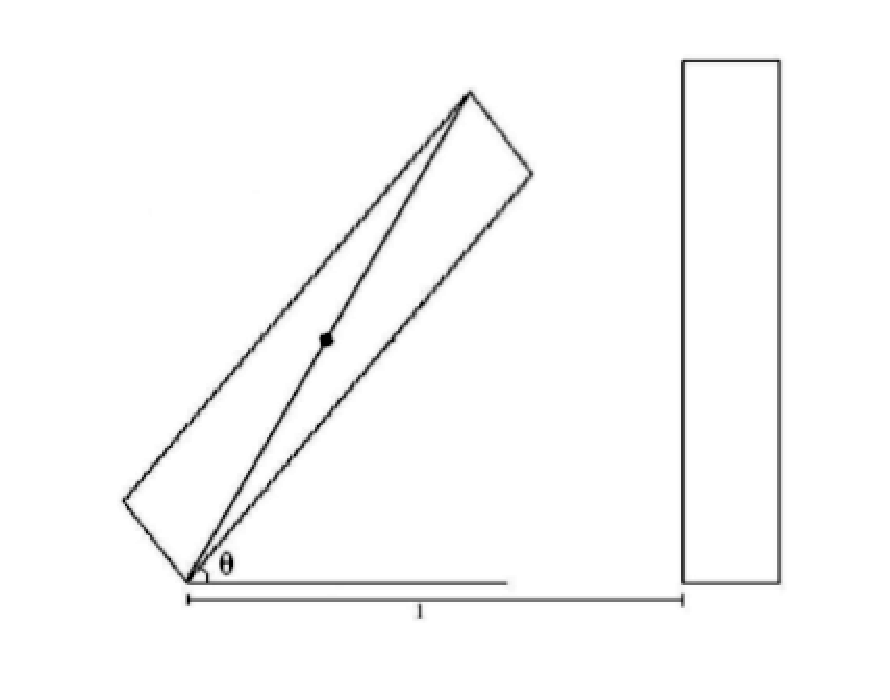
\includegraphics[width=7cm]{domin}
\end{figure}

Koellhoffer et al. \cite{FallingDominoes} proceed to find the total energy for the falling domino using simple geometric constructions.Note that the domino makes angle $\theta$ in $radians$ with the horizontal at a moment in time:
\begin{itemize}
	\item The potential energy of the falling domino $U$ in $J$ is:
\begin{equation}
U = mg\left( \frac{T}{2} \cos\theta + \frac{h}{2}\sin\theta \right)
\end{equation}
	where $g$ is the acceleration due to gravity in $metres/{sec}^2$.
	\item Let $I$ be the domino's moment of inertia in $kilogram-metre^2$ about it's center of mass and $t$ is time in $seconds$. Therfore,
		\begin{equation}
			I = \frac{1}{12} m \left( h^2 + T^2 \right)
		\end{equation}
		and
		\begin{equation}
			v = \frac{T}{2}{d\theta \over dt}
		\end{equation}
	\item The kinetic energy $K$ in $J$ is:
	\begin{equation}
		K = \frac{1}{2} mv^2 + \frac{1}{2}I \left({d\theta \over dt}\right)^2
	\end{equation}
	where $v$ is the tangential velocity of the domino about it's center of mass in $metres/sec$
\end{itemize}

Combining all these equations, we get the total energy of the domino $E$ in $J$
\begin{equation}
	E = K + U
\end{equation}

\begin{equation}
	E = mg \left( \frac{T}{2} \cos\theta + \frac{h}{2} \sin\theta \right) + \frac{1}{6} m \left({d\theta \over dt}\right)^2 \left( h^2 + T^2 \right) 
\end{equation}

\subsection{The revolving platform}

The platform holds a heavy ball on top of it and is hinged about it's center of mass. The other rod which rises due to the balls falling in the basket on the other side of the pulley, hits the hinged platform at one end. Due to this, a force $F$ is imparted. Since the platform cannot undergo any translational motion,
it starts rotating due to the torque it has received at one end of the rod. This causes the rod to start rotating with an angular acceleration $\alpha$. 
\begin{figure}[h!]
\caption{The horizontal revolving platform}
\centering
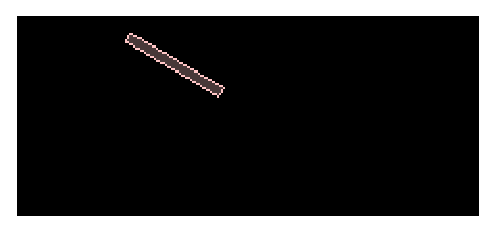
\includegraphics[width=10cm,scale=2]{rotplatform}
\end{figure}
The moment of inertia of this rod hinged about it's center is $\frac{1}{2}m l^2$ \cite{Wiki}
\begin{equation}
\frac{F l}{2} = \frac{1}{2}m l^2 \alpha
\end{equation}
where $F$ is the force as mentioned above in $Newton$, $l$ is length of the rotating rod in $metres$, $m$ is the mass of the rotating rod in $kilograms$ and $\alpha$ is the angular acceleration it acquires in $radians/{sec}^2$

\section{Conclusions}
Hopefully, the reader has by now got some insight into the complicated yet simplistic physics involved in the breathtaking Rube Goldberg Machines.
\\
To summarise, 
\begin{enumerate}
	\item We started out with the velocity with which the pendulum bob hits the first domino which is approximately the same as the velocity which the domino acquires.

	\item We then go on to find the total energy that the toppling domino has while toppling using simple geometric construction, \emph{law of conservation of energy} and \emph{law of conservation of angular momentum.}

	\item We finally observe the hinged platform which gets an initial torque due to the rising rod that hits it.We then go on to find the angular acceleration $\alpha$  with which this platform starts rotating.
\end{enumerate}
\bibliographystyle{plain}
\bibliography{refs}
\end{document}
